\chapter{Tecnología}
\section{Introducción}
El principal elemento de estructura activa de la Capa de Tecnología es el nodo. Este elemento se utiliza para modelar entidades estructurales en esta capa. Modela estrictamente el aspecto estructural de un sistema: su comportamiento está modelado por una relación explícita con el elemento de comportamiento. Una interfaz de tecnología es el lugar (lógico) en el que se puede acceder a los servicios tecnológicos ofrecidos por un nodo mediante otros nodos o mediante componentes de aplicación de la Capa de Aplicación. Los nodos vienen en varias presentaciones, incluyendo software de dispositivos y sistemas. Un dispositivo modela un recurso físico computacional, sobre el cual se pueden desplegar artefactos para su ejecución. El software de sistema es un componente de software de infraestructura que se ejecuta en un dispositivo. Típicamente, un nodo consiste en un número de subnodos; por ejemplo, un dispositivo como un servidor y software de sistema para modelar el sistema operativo.
Las interrelaciones de los componentes de la Capa de Tecnología están formadas principalmente por la infraestructura de comunicación. La trayectoria modela la relación entre dos o más nodos, a través de la cual estos nodos pueden intercambiar información. La realización física de un trayecto se modela con una red de comunicación; es decir, un medio de comunicación físico entre dos o más dispositivos (u otras redes).

\begin{itemize}
	\item Un nodo representa un recurso computacional o físico que alberga, manipula o interactúa con otros recursos computacionales o físicos.
	\item Un dispositivo es un recurso físico TI en el que se pueden almacenar o desplegar programas y artefactos del sistema para su ejecución.
	\item El software del sistema representa el software que proporciona o contribuye a un entorno para almacenar, ejecutar y utilizar el software o los datos desplegados en él.
	\item Una colaboración tecnológica representa un agregado de dos o más nodos que trabajan juntos para realizar un comportamiento tecnológico colectivo.
	\item Una interfaz tecnológica representa un punto de acceso donde los servicios tecnológicos ofrecidos por un nodo
	se puede acceder.
	\item Una red de comunicaciones representa un conjunto de estructuras que conectan sistemas informáticos u otros dispositivos electrónicos para la transmisión, el enrutamiento y la recepción de datos.
\end{itemize}

%\newpage

\section{Metamodelo}
\begin{figure}[h!]
	\centering
	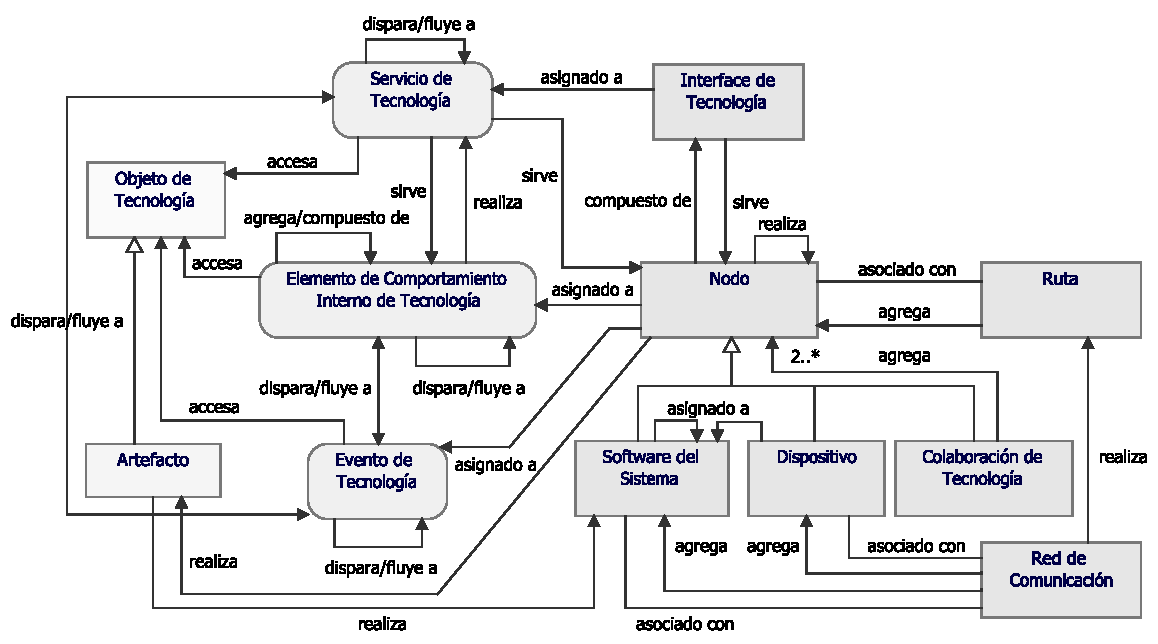
\includegraphics[width=0.9\linewidth]{imgs/meta/Tecnologia}
	\caption{Metamodelo Tecnologia}
	\label{fig:mTech}
\end{figure}

La figura \ref{fig:mTech} da una visión general de los elementos de la Capa de Tecnología y sus relaciones. Siempre que sea aplicable, la concepción se extrae de la analogía con las Capas de Negocio y Aplicación. La Capa de Tecnología se utiliza típicamente para modelar la arquitectura tecnológica de la empresa, definida por el marco TOGAF como: "la estructura e interacción de los servicios de la plataforma, y los componentes tecnológicos lógicos y físicos".

\newpage
\section{Punto de Vista de Implmenetación y Migración}
\newpage
\chapter{Tecnologia}
\section{Introduccion}
contenido...

\newpage

\section{Metamodelo}
\begin{figure}[h!]
	\centering
	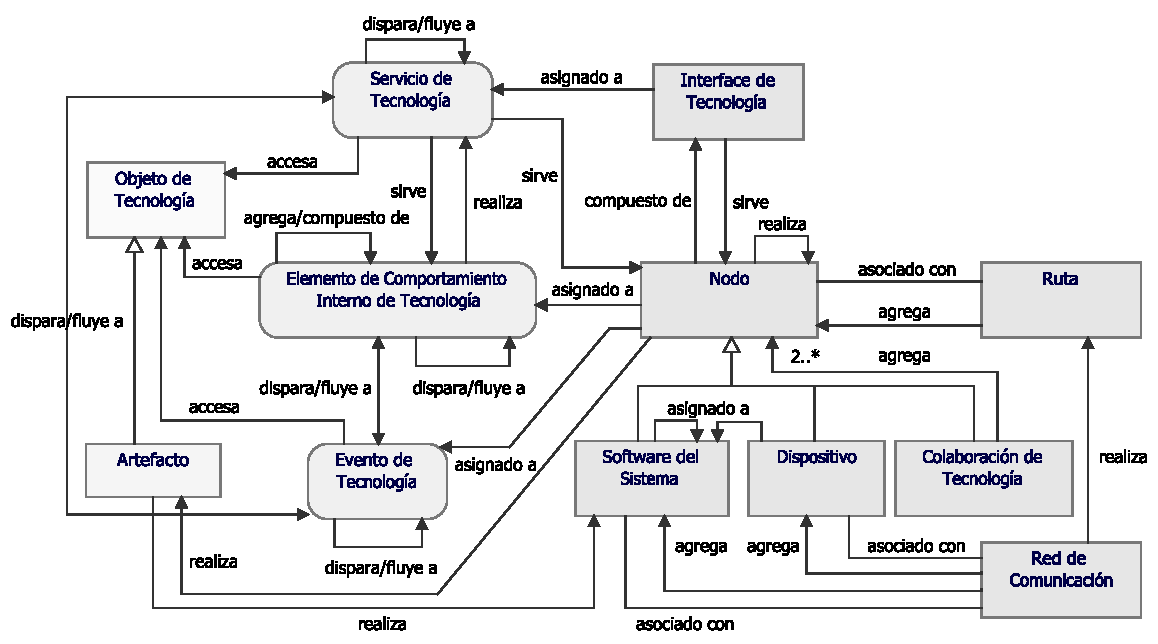
\includegraphics[width=0.9\linewidth]{imgs/meta/Tecnologia}
	\caption{Metamodelo Tecnologia}
\end{figure}

descripcion....

\newpage

\section{Punto de Vista de Implementacion y Despliegue}
contenido....
\subsection{Modelo de Implementacion y Despliegue}
\begin{figure}[h!]
	\centering
	\includegraphics[width=.5\linewidth]{imgs/modelo/Implementacion}
	\caption{Modelo Implementacion y Despliegue}
\end{figure}
descripcion...

\newpage

\subsection{Caso  de Implementacion y Despliegue}
\begin{figure}[h!]
	\centering
	\includegraphics[width=.5\linewidth]{imgs/caso/Implementacion}
	\caption{Caso Implementacion y Despliegue}
\end{figure}
descripcion...

\newpage
\newpage
\section{Punto de Vista de Uso de Tecnología}

El punto de vista de la utilización de la tecnología muestra cómo las aplicaciones son apoyadas por la tecnología de software y hardware: los servicios tecnológicos son suministrados por los dispositivos; el software y las redes del sistema son suministrados a las aplicaciones. Este punto de vista desempeña un papel importante en el análisis del rendimiento y la escalabilidad, ya que relaciona la infraestructura física con el mundo lógico de las aplicaciones. Es muy útil para determinar los requisitos de rendimiento y calidad de la infraestructura en función de las exigencias de las diversas aplicaciones que la utilizan.

\subsection{Modelo de Uso de la Tecnología}
\begin{figure}[h!]
	\centering
	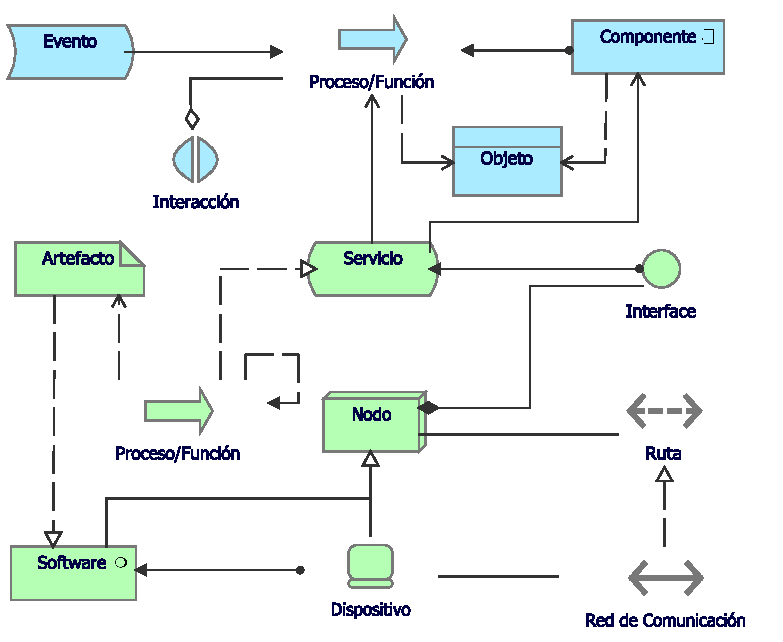
\includegraphics[width=.8\linewidth]{imgs/modelo/UsoTecnologia.pdf}
	\caption{Modelo Implementacion y Despliegue}
\end{figure}

Una función tecnológica describe el comportamiento interno de un nodo; para el usuario de un nodo que realiza una función tecnológica, esta función es invisible. Si su comportamiento es expuesto externamente, esto se hace a través de uno o más servicios tecnológicos. Una función tecnológica se abstrae de la forma en que se implementa. Sólo se especifica el comportamiento necesario. Una función de tecnología puede realizar servicios de tecnología. Los servicios tecnológicos de otras funciones tecnológicas pueden servir a las funciones tecnológicas. Una función tecnológica puede acceder a los objetos tecnológicos. Se puede asignar un nodo a una función tecnológica (lo que significa que el nodo realiza la función tecnológica). El nombre de una función tecnológica debe ser preferentemente un verbo sustantivado.

%\newpage

\subsection{Caso  de  Uso de la Tecnología}
\begin{figure}[h!]
	\centering
	\includegraphics[width=.7\linewidth]{imgs/caso/Implementacion}
	\caption{Caso Implementacion y Despliegue}
\end{figure}
descripcion...
\newpage
\section{Punto de Vista Estructura de Información}
contenido....
\subsection{Modelo de Implementacion y Despliegue}
\begin{figure}[h!]
	\centering
	\includegraphics[width=.5\linewidth]{imgs/modelo/Implementacion}
	\caption{Modelo Implementacion y Despliegue}
\end{figure}
descripcion...

\newpage

\subsection{Caso  de Implementacion y Despliegue}
\begin{figure}[h!]
	\centering
	\includegraphics[width=.5\linewidth]{imgs/caso/Implementacion}
	\caption{Caso Implementacion y Despliegue}
\end{figure}
descripcion...
\newpage
\section{Punto de Vista de Realización de Servicio}
contenido....
\subsection{Modelo de Implementacion y Despliegue}
\begin{figure}[h!]
	\centering
	\includegraphics[width=.5\linewidth]{imgs/modelo/Implementacion}
	\caption{Modelo Implementacion y Despliegue}
\end{figure}
descripcion...

\newpage

\subsection{Caso  de Implementacion y Despliegue}
\begin{figure}[h!]
	\centering
	\includegraphics[width=.5\linewidth]{imgs/caso/Implementacion}
	\caption{Caso Implementacion y Despliegue}
\end{figure}
descripcion...
\newpage
\subsection{Físico}

Estos se basan en la Capa de Tecnología. No se definen elementos de comportamiento físico separados.  Más bien, los elementos de comportamiento de la Capa de Tecnología (función de la tecnología, proceso, interacción, servicio y evento) se usan para modelar el comportamiento de todos los nodos, incluyendo el equipo físico. Dado que el equipo muy a menudo estará controlado por computadora o tendrá una estrecha relación con la tecnología de la información (piense también en los sensores, Internet de las cosas), su comportamiento puede describirse de manera integral utilizando los conceptos de comportamiento de la tecnología existente.

\newpage
\subsubsection{Elementos de la Estructura}

\begin{longtable}{|c| c| c|}
	\hline
	Concepto & Descripción & Representación \\ \hline
	Facilidad
	&
	\begin{tabular}{p{6cm}p{3cm}}
		Representa un recurso físico que tiene la capacidad de
		facilitar (por ejemplo, albergar o ubicar) el uso de equipos. Por lo general, se utiliza para modelar fábricas, edificios o construcciones al aire libre
	\end{tabular} 
	& 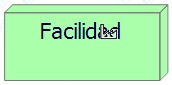
\includegraphics[width=0.1\linewidth, height=0.05\textheight]{imgs/conceptos/fisico/facilidad}
	\\
	\hline 
	Equipo
	& 
	\begin{tabular}{p{6cm}p{3cm}}
		El equipo comprende todos los elementos de procesamiento activos que llevan a cabo procesos físicos en los que se utilizan o transforman materiales.
	\end{tabular} 
	& 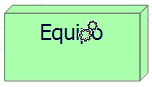
\includegraphics[width=0.1\linewidth, height=0.05\textheight]{imgs/conceptos/fisico/equipo}
	\\
	\hline
	Red de distribución
	&
	\begin{tabular}{p{6cm}p{3cm}} 
		Representa la distribución física o la infraestructura de transporte. Encarna la realización física de las rutas lógicas entre nodos. Una red de distribución conecta dos o más nodos. Una red de distribución puede realizar uno o más caminos.
	\end{tabular} 
	& 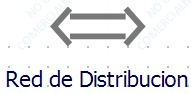
\includegraphics[width=0.1\linewidth, height=0.05\textheight]{imgs/conceptos/fisico/redDistribucion}
	\\
	\hline
	Material
	&
	\begin{tabular}{p{6cm}p{3cm}}  
		El material representa materia física tangible, con atributos como tamaño y peso. Suele utilizarse para modelar materias primas y productos físicos, y también fuentes de energía como el combustible.
	\end{tabular}
	& 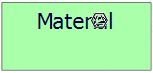
\includegraphics[width=0.1\linewidth, height=0.05\textheight]{imgs/conceptos/fisico/material}
	\\
	\hline
\end{longtable}
\newpage
\section{Punto de Vista de Capas}

El punto de vista por capas muestra las diferentes capas y aspectos de la arquitectura empresarial en un modelo. Existen dos categorías de capas, capas dedicadas y capas de servicio. Las capas son resultado de la relación de “agrupación” para un particionado natural de todo el conjunto de objetos y relaciones que pertenecen al modelo. La infraestructura, la aplicación, los procesos y los actores/roles pertenecen a la primera categoría. El principio estructural es que cada capa dedicada expone por medio de una relación de “realización” una capa de servicios, las cuales serán “usadas por” la siguiente capa dedicadas. A partir de esto se puede separar la estructura interna y la organización de cada capa dedicada de su comportamiento externo observable expresado como el servicio que esa capa dedicada realiza. 

\subsection{Modelo de Capas}
\begin{figure}[h!]
	\centering
	\includegraphics[width=.5\linewidth]{imgs/modelo/Implementacion}
	\caption{Modelo de Capas}
\end{figure}

El modelo de capas muestra como los servicios de negocio, aplicación e infraestructura son integrados por medio de sus modelos intermedios: Se muestran los servicios de negocio principales y los procesos de negocio que los realizan, estos procesos están asociados con servicios de aplicación específicos que a su vez son realizados por componentes de aplicación definidos para la arquitectura del sistema de software. Los componentes se encuentran soportados en servicios de infraestructura realizados por nodos de infraestructura y aplicaciones de software concretas.

\newpage

\subsection{Caso  de Capas}
\begin{figure}[h!]
	\centering
	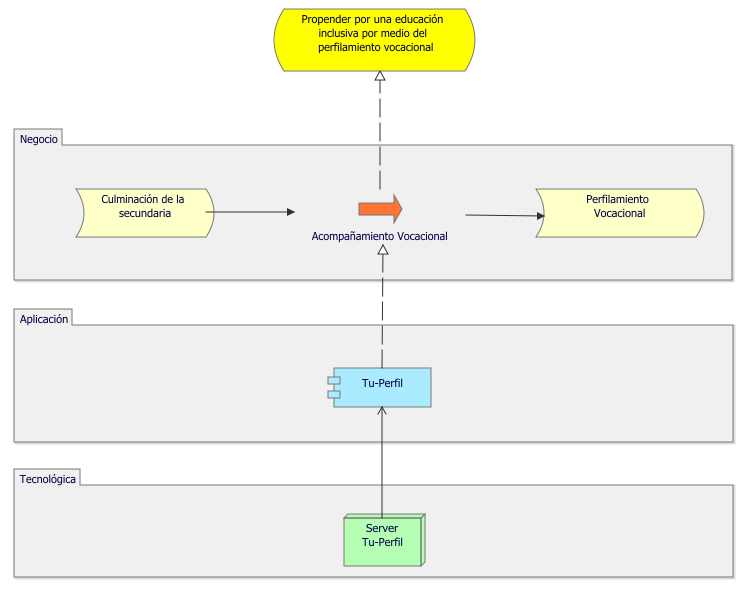
\includegraphics[width=.5\linewidth]{imgs/caso/CapasTuPerfil}
	\caption{Caso de Capas}
\end{figure}

Para el caso del proyecto Tu-Perfil, el punto de vista de capas inicia con el objetivo central del proyecto Tu-Perfil, el cual es propender por una educación inclusiva por medio del perfilamiento vocacional y se conecta con tres capas fundamentales en el proceso de construcción del proyecto, estas capas son: la capa de negocio en la cual se especifica lo más relevante trabajado en esos puntos de vista pertenencientes a la capa de negocio contando con el proceso principal del acompañamiento vocacional precedido por la culminación de la secundaria y lo sucede el perfilamiento vocacional. Sigue la capa de aplicación con el paquete principal de Tu-Perfil y la capa tecnológica con el servidor Tu-Perfil.

\clearpage